\documentclass[main.tex]{subfiles}
\begin{document}
\section{Question 1}
Create a new system call \texttt{wait2}, which extends the \texttt{wait} system call.
\\
\texttt{int wait2(int *wtime, int *rtime, int *iotime)}

Where the three arguments are pointers to integers to which the wait2 function will assign:
\begin{enumerate}
  \item The aggregated number of clock ticks during which the process waited
    (was able to run but did not get CPU)
  \item The aggregated number of clock ticks during which the process was
    running
  \item The aggregated number of clock ticks during which the process was
    waiting for I/O (was not able to run).
\end{enumerate}
The \texttt{wait2} function shall return the pid of the child process caught or -1 upon failure

\lstinputlisting[style=codeStyleC]{listings/1.c}
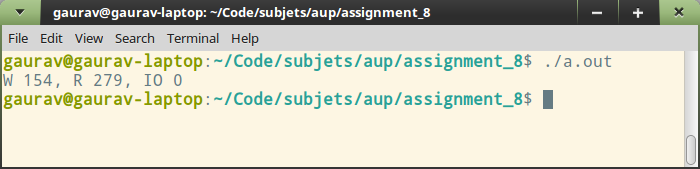
\includegraphics[width=\textwidth]{figures/1_output.png}
\end{document}
